% Lower array: the faint overlay and hatched superscript retain their actual strokes.
% A question at either graphic locus marks the unresolved character identification.
\diagram{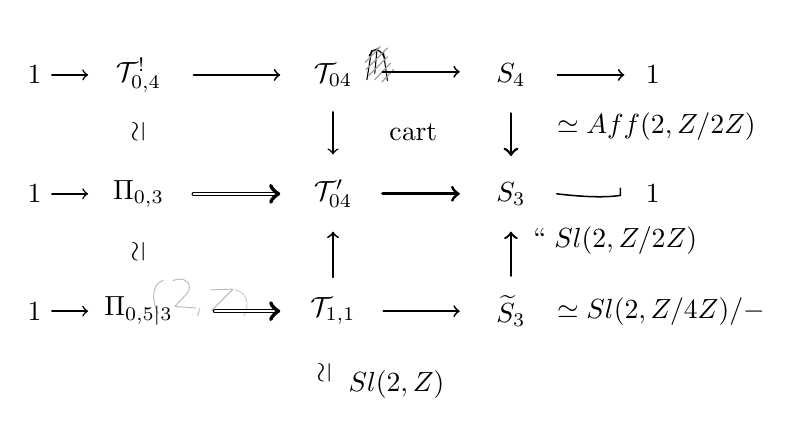
\begin{tikzpicture}[x=1cm,y=1cm,line cap=round,line join=round]
% Pale overwritten span beside the lower Pi; drawn before the dark label and shaft.
\draw[gray!55,line width=.35pt] (1.63,-2.61)..controls(1.49,-2.65)and(1.48,-2.87)..(1.57,-3.03);
\draw[gray!55,line width=.35pt] (1.76,-2.61)..controls(1.91,-2.55)and(2.02,-2.66)..(1.94,-2.77)--(1.78,-2.94)--(2.05,-2.96);
\draw[gray!50,line width=.35pt] (2.10,-2.96)--(2.07,-3.06);
\draw[gray!55,line width=.35pt] (2.24,-2.73)--(2.52,-2.72)--(2.25,-2.99)--(2.54,-2.99);
\draw[gray!45,line width=.3pt] (2.55,-2.73)..controls(2.69,-2.76)and(2.74,-2.90)..(2.66,-3.06);
\node[inner sep=0pt] at (2.79,-3.19) {$\unsure{\phantom{A}}$};
\node[inner sep=0pt] (u0) at (0,0) {$1$};
\node[inner sep=0pt] (u1) at (1.32,0) {$\mathcal T_{0,4}^{!}$};
\node[inner sep=0pt] (u2) at (3.79,0) {$\mathcal T_{04}$};
\node[inner sep=0pt] (u3) at (6.05,0) {$\unsure{\mathfrak S}_4$};
\node[inner sep=0pt] (u4) at (7.85,0) {$1$};
\node[inner sep=0pt] (m0) at (0,-1.51) {$1$};
\node[inner sep=0pt] (m1) at (1.32,-1.51) {$\Pi_{0,3}$};
\node[inner sep=0pt] (m2) at (3.79,-1.51) {$\mathcal T'_{04}$};
\node[inner sep=0pt] (m3) at (6.05,-1.51) {$\unsure{\mathfrak S}_3$};
\node[inner sep=0pt] (m4) at (7.85,-1.51) {$1$};
\node[inner sep=0pt] (l0) at (0,-3.00) {$1$};
\node[inner sep=0pt] (l1) at (1.32,-3.00) {$\Pi_{0,\unsure{5|3}}$};
\node[inner sep=0pt] (l2) at (3.79,-3.00) {$\mathcal T_{1,1}$};
\node[inner sep=0pt] (l3) at (6.05,-3.00) {$\widetilde{\unsure{\mathfrak S}}_3$};
\draw[->,line width=.55pt] (.22,0)--(.68,0);
\draw[->,line width=.65pt] (2.02,0)--(3.12,0);
% The upper middle arrow begins in the crossed raised cluster.
\draw[line width=.45pt] (4.25,.24)..controls(4.31,.39)and(4.42,.30)..(4.45,.20);
\draw[line width=.4pt] (4.28,.31)--(4.22,-.06) (4.35,.34)--(4.32,.02) (4.43,.29)--(4.48,-.07);
\draw[gray!75,line width=.45pt] (4.20,.16)--(4.39,.36) (4.21,.07)--(4.48,.34) (4.24,-.01)--(4.48,.23) (4.32,-.06)--(4.52,.15) (4.41,-.09)--(4.56,.07);
\node[inner sep=0pt] at (4.53,.48) {$\unsure{\phantom{A}}$};
\draw[->,line width=.65pt] (4.42,.04)--(5.40,.04);
\draw[->,line width=.65pt] (6.64,0)--(7.49,0);
\draw[->,line width=.55pt] (.22,-1.51)--(.68,-1.51);
\draw[double,double distance=.65pt,->,line width=.45pt] (2.02,-1.51)--(3.12,-1.51);
\draw[->,line width=1.1pt] (4.42,-1.51)--(5.40,-1.51);
% The middle terminal connector has a blunt upturned end, without a supplied head.
\draw[line width=.55pt] (6.63,-1.51)..controls(6.98,-1.55)and(7.24,-1.56)..(7.44,-1.53)--(7.44,-1.44);
\draw[->,line width=.55pt] (.22,-3.00)--(.68,-3.00);
\draw[double,double distance=.65pt,->,line width=.45pt] (2.29,-3.00)--(3.12,-3.00);
\draw[->,line width=.65pt] (4.43,-3.00)--(5.40,-3.00);
\draw[->,line width=.55pt] (3.79,-.47)--(3.79,-1.01);
\draw[->,line width=1pt] (6.05,-.49)--(6.05,-1.03);
\draw[->,line width=.65pt] (3.79,-2.57)--(3.79,-1.99);
\draw[->,line width=.85pt] (6.05,-2.55)--(6.05,-1.99);
\node[inner sep=0pt] at (1.32,-.72) {\rotatebox{90}{$\simeq$}};
\node[inner sep=0pt] at (1.32,-2.24) {\rotatebox{90}{$\simeq$}};
\node[inner sep=0pt] at (4.81,-.72) {cart};
\node[anchor=west,inner sep=0pt] at (6.63,-.65) {$\simeq\operatorname{Aff}(2,\mathbb Z/2\mathbb Z)$};
\node[anchor=west,inner sep=0pt] at (6.30,-2.10) {`` $\operatorname{Sl}(2,\mathbb Z/2\mathbb Z)$};
\node[anchor=west,inner sep=0pt] at (6.63,-3.00) {$\simeq\operatorname{Sl}(2,\mathbb Z/4\mathbb Z)/-$};
\node[inner sep=0pt] at (3.68,-3.78) {\rotatebox{90}{$\simeq$}};
\node[anchor=west,inner sep=0pt] at (3.98,-3.93) {$\operatorname{Sl}(2,\mathbb Z)$};
\end{tikzpicture}}
